\chapter{La società della conoscenza}
\thispagestyle{chapterInit}
In questo capitolo andremo ad analizzare il concetto di ``società della conoscenza'' e le nuove leggi che regolano questa società. Inoltre andremo ad analizzare il \textit{\textbf{Hype Cycle}} di \textbf{Gartner} e il \textit{\textbf{Long Tail}} di \textbf{Anderson}.
\section{Introduzione}
    \paragraph{Cos'è una ``società della conoscenza''} Il concetto di ``\textbf{società della conoscenza}'' si riferisce ad un modello di società nel quale la \textbf{conoscenza}, l'\textbf{informazione} e l'\textbf{innovazione} diventano i principali \textbf{mezzi della crescita economica e dello sviluppo sociale}. In questo tipo di società viene ``premiato'' chi ha la \textbf{capacità di apprendere, di innovare} e di \textbf{adattarsi ai rapidi cambiamenti tecnologici}.
    \paragraph{Perchè è importante?} La \textbf{conoscenza} è importante perché in una economia basata su questa la ricchezza e il potere sono determinati dalla \textbf{capacità di creare}, inoltre la \textbf{innovazione e competitività} è essenziale e la nuova idea domina i mercati. Altro asset importante è il \textbf{capitale umano e l'istruzione} in quanto le persone ben formate sono in grado di creare valore. La \textbf{globalizzazione e interconnessione} sono altri fattori importanti in quanto la conoscenza è un bene che si diffonde rapidamente e facilmente. Infine anche lo \textbf{sviluppo sostenibile} è importante in quanto la conoscenza permette di trovare soluzioni a problemi ambientali.
\section{Nuove leggi della società della conoscenza}
    In questa sezione sono analizzate le nuove leggi che regolano la società della conoscenza, ovvero la \textbf{legge di Moore}, la \textbf{legge di Sarnoff}, la \textbf{legge di MetCalfe} e la \textbf{legge di Reed}.
    \subsection{Leggi di Moore}
        Di seguito sono analizzate le due leggi di Moore collegate al mondo dell'informatica.
        \subsubsection{Prima legge di Moore}
            La \textbf{legge di Moore} è un'osservazione fatta da \textbf{Gordon Moore} nel 1965
            \begin{definition}[Prima legge di Moore]
                La \textbf{densità di transistor} nei circuiti integrati raddoppia ogni $18$ mesi.
            \end{definition}
            \paragraph{Limiti} I limiti della prima legge di Moore riguardano il raggiungimento dei limiti fisici della materia.
            \paragraph{Conseguenze} 
            Questo comporta che la potenza di calcolo dei computer raddoppia ogni $18$ mesi. Come conseguenza tale legge suggerisce un \textbf{aumento esponenziale} della potenza di calcolo dei computer, portando ad un \textbf{aumento della velocità} e della \textbf{capacità di memorizzazione} dei computer. Questo ha portato ad un \textbf{aumento della diffusione} dei computer e ad una \textbf{riduzione dei costi}.
        \subsubsection{Seconda legge di Moore}
            La \textbf{seconda legge di Moore} è una osservazione eseguita da \textbf{Gordon Moore} nel 1975, successivamente integrata da altri autori.
            \begin{definition}[Seconda legge di Moore]
                L'investimento per realizzare una nuova tecnologia di microprocessori cresce in maniera esponenziale con il tempo.
            \end{definition}
            \paragraph{Conseguenze} Questa legge implica che per aumentare la potenza di calcolo dei computer è necessario un \textbf{investimento sempre maggiore}. Questo ha portato ad un \textbf{aumento dei costi} per la realizzazione di nuove tecnologie.\newline Questi effetti fanno sì che le società che si possono permettere di investire sono sempre meno e quelle che da sole non riescono ad investire si uniscono. Effetto economico di questa legge è l'aumento del rischio degli investimenti. Difatti la probabilità di fallimento di una nuova azienda si incrementa con il tempo.
    \subsection{Leggi di Sarnoff, MetCalfe, Reed}
        Dopo aver analizzato le leggi di Moore riguardanti il mondo dell'informatica, analizziamo le leggi di Sarnoff, MetCalfe e Reed che riguardano il mondo delle reti nella società della conoscenza.
        \subsubsection{Legge di Sarnoff}
            La \textbf{legge di Sarnoff} è un'osservazione fatta da \textbf{David Sarnoff} nel 1950 la quale interessa il valore di un sistema di comunicazione del tipo \textit{broadcast}.
            \begin{definition}[Legge di Sarnoff]
                Il valore $V$ di una rete di broadcasting è direttamente proporzionale al numero $N$ di utenti della rete. 
                $$ V = N $$
            \end{definition}
            \paragraph{Conseguenze} Il valore della rete aumenta con il numero di utenti.
        \subsubsection{Legge di MetCalfe}
            La \textbf{legge di MetCalfe} è un'osservazione fatta da \textbf{Robert MetCalfe} nel 1980 la quale interessa il valore di un sistema di comunicazione del tipo \textit{peer-to-peer} ovvero una rete di relazione sociale. Esempi di reti di relazione sociale sono la rete telefonica o il sistema di fax per le quali è possibile una comunicazione bidirezionale ma limitata ad 1-1.
            \begin{definition}[Legge di MetCalfe]
                Il valore $ V $ di un sistema di comunicazione cresce con il quadrato del numero di utenti $ N $ della rete.
                $$ V = N^2 - N $$
            \end{definition}
            \paragraph{Implicazione} La connessione di reti indipendenti crea un valore più elevato rispetto alla somma del valore delle singole reti. Questa legge è molto legata al successo di internet quando questa si basava sulla esistente rete telefonica.
        \subsubsection{Legge di Reed}
            La \textbf{legge di Reed} è un'osservazione fatta da \textbf{David Reed} nel 1999 la quale interessa il valore di un sistema di comunicazione nella quale è possibile la comunicazione tra più di due utenti o gruppi di utenti. Esempi di reti di relazione sociale sono i social network o i forum.
            \begin{definition}[Legge di Reed]
                L'utilità dele grandi reti, formate da reti di reti (con particolare riferimento alle reti di relazione sociale) cresce esponenzialmente con il numero di nodi. $$ V = 2^N - N - 1 $$
            \end{definition}
            \paragraph{Conseguenze} Questa legge implica che il valore di una rete sociale cresce esponenzialmente con il numero di nodi. Questo è dovuto al fatto che con ogni nodo si possono creare nuovi sottogruppi di nodi.
        \subsubsection{Conclusione leggi di Sarnoff, MetCalfe, Reed}
            Se si distribuisce un solo contenuto allora si ha una crescita lineare del valore, se si attivano transizione per il commercio elettronico si ha una crescita quadratica del valore, se si crea una comunità si ha una crescita esponenziale del valore. \newline Per chi investe è meglio puntare sulla legge di Reed in quanto il valore cresce esponenzialmente con il numero di nodi.
\section{Hype Cycle di Gartner}
    L'\textbf{Hype Cycle} è un modello sviluppato da \textbf{Gartner} (società) che rappresenta la \textbf{maturità, l'adozione e l'applicazione delle tecnologie emergenti}. Il modello è rappresentato da un grafico che mostra la \textbf{curva di hype} di una tecnologia, ovvero la \textbf{fase di crescita e declino} di una tecnologia.
    \subsection{La curva della domanda}
        Prima di analizzare l'\textbf{Hype Cycle} è importante conoscere la \textbf{curva della domanda} la quale rappresenta come un determinato prodotto e/o tecnologia viene adottato dal mercato.
        \paragraph{Componenti della curva} 
            La curva è composta da tre picchi di acquisto: i \textbf{pionieri}, la \textbf{maggioranza} e i \textbf{ritardatari}.\newline 
            I \textbf{pionieri} sono quella cerchia ristretta di persone che sono disposte a comprare un prodotto appena uscito anche a costi elevati. La \textbf{maggioranza} è quella cerchia di persone che comprano un prodotto quando il prezzo è ragionevole ma pretendono tecnologie semplici e facili da usare e sono sensibili ai trend creati dai pionieri. Infine i \textbf{ritardatari} sono coloro che comprano un prodotto quando ormai è diventato un bene di uso comune e non si possono esimere dall'acquisto per rimanere competitivi sul mercato, questi sono molto prudenti e non amano rischiare inoltre la loro preoccupazione principale è il costo.
            \begin{figure}[H]
                \centering
                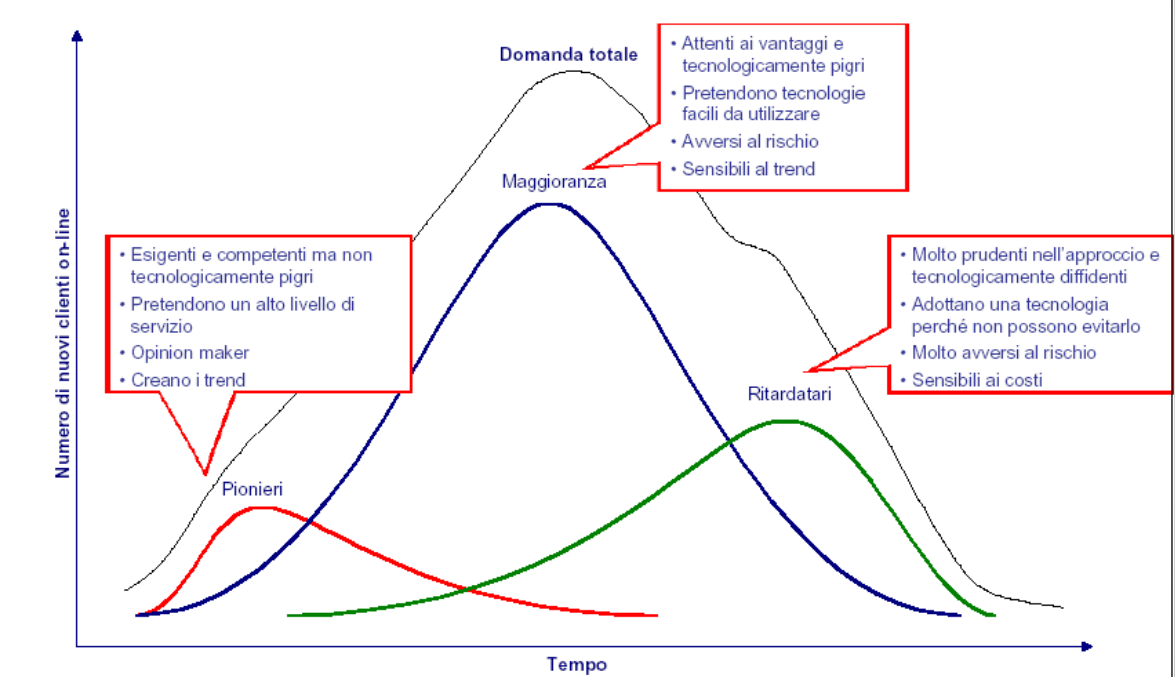
\includegraphics[width=0.5\textwidth]{01/graficoDomanda.png}
                \caption{Curva della domanda}
            \end{figure}
    
    \subsection{Hype Cycle}
        Il grafico di seguito illustra la \textbf{curva di hype} di una tecnologia, ovvero la \textbf{fase di crescita e declino} di una tecnologia. Questo grafico è importante per capire come una nuova tecnologia viene richiesta ed adottato dal mercato.
        \subsubsection{Le fasi}
            Questa curva ha diversi alti e bassi:
            \begin{enumerate}
                \item \textbf{Innovazione} è la fase in cui la tecnologia viene presentata al mercato e le prime startup iniziano a sviluppare prodotti basati su questa tecnologia.
                \item \textbf{Crescita esponenziale} è la fase in cui la tecnologia inizia a venire seguita da un numero sempre maggiore di persone e il mercato potenziale dietro a questa tecnologia inizia a crescere. I mass media iniziano a parlare di questa tecnologia. I primi prodotti basati su questa tecnologia iniziano ad essere venduti ad un costo molto elevato.
                \item \textbf{Picco delle aspettative inflazionate} è la fase in cui la tecnologia raggiunge il suo picco di interesse e le aspettative sono molto alte. In questa fase la tecnologia è vista come la soluzione a tutti i problemi.
                \item \textbf{Declino} è la fase in cui la tecnologia non riesce a soddisfare le aspettative e il mercato inizia a perdere interesse, in quanto la tecnologia non è in grado di risolvere i problemi del suo punto di massimo.
                \item \textbf{Risalita della produttività} è la fase in vengono realizzati la seconda/terza generazione dei prodotti basati su questa tecnologia e il mercato inizia a capire come utilizzare questa tecnologia in modo efficace. In questa fase la tecnologia inizia a diventare un bene di uso comune.
                \item \textbf{Piatto di produttività} è la fase in cui la tecnologia è diventata un bene di uso comune e il mercato inizia a saturarsi. Qui la tecnologia viene usata per risolvere problemi specifici ma non è più vista come la soluzione a tutti i problemi (20/30 \% del mercato rispetto al picco).
            \end{enumerate}
            \begin{figure}[H]
                \centering
                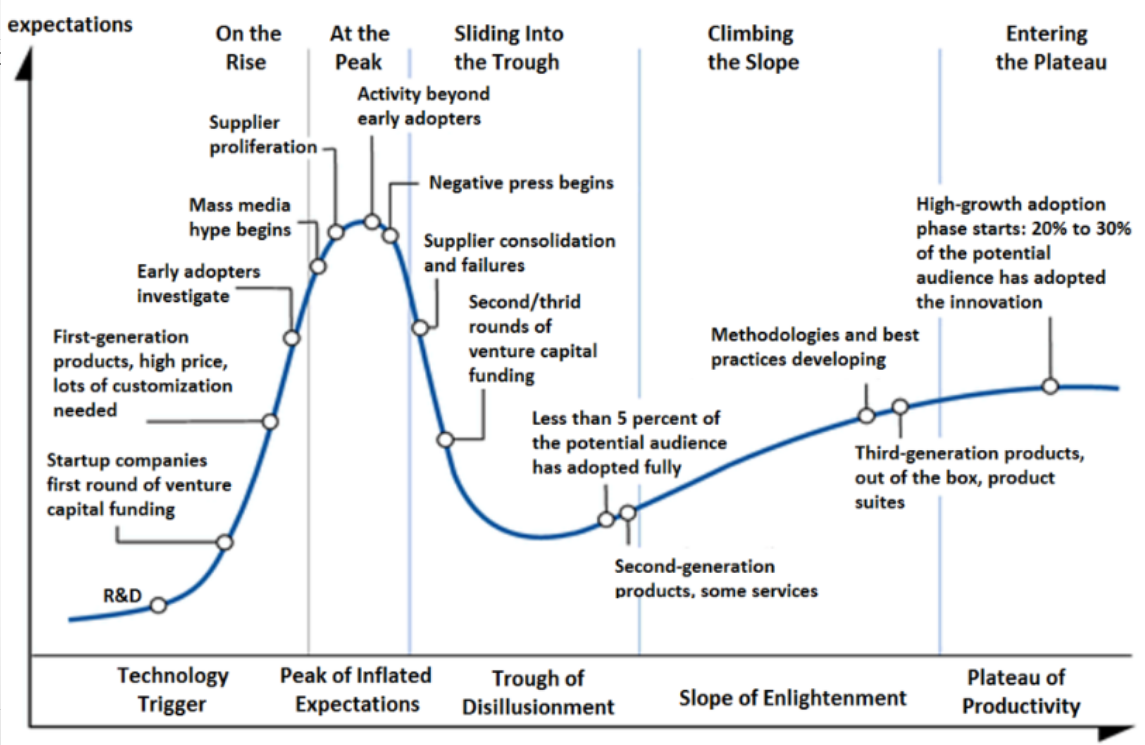
\includegraphics[width=0.5\textwidth]{01/hypeCycle.png}
                \caption{Curva di hype}
            \end{figure}
            Qualche volta però la tecnologia non riesce a riprendersi dal declino, vengono quindi proposte altre due curve con fasi che si sostituiscono alle fasi 5 e 6:
            \begin{enumerate}
                \item[5.] \textbf{Cimitero delle tecnologie} è la fase in cui la tecnologia non riesce a riprendersi dal declino e viene abbandonata.
                \item[5.] \textbf{Palude di uso comune} è la fase in cui la tecnologia è diventata un bene di uso comune ma non riesce a trovare nuove applicazioni e il mercato è molto più ristretto, il prodotto viene usato solo da una cerchia ristretta di persone.
            \end{enumerate}
            \begin{figure}[H]
                \centering
                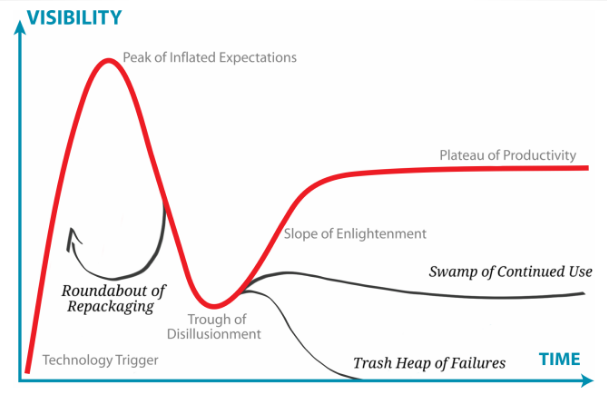
\includegraphics[width=0.5\textwidth]{01/hypeCycleAlt.png}
                \caption{Curva di hype con fasi alternative}
            \end{figure}
    \subsection{Magic Quadrant di Gartner}
        Il \textbf{Magic Quadrant} è un modello sviluppato da \textbf{Gartner} che permette di valutare le \textbf{aziende} in base alla loro \textbf{completezza della visione} e alla loro \textbf{abilità di esecuzione}. Questo modello è importante per capire come un'azienda si posiziona rispetto ai suoi concorrenti e per capire quali sono i punti di forza e di debolezza di un'azienda.
        \subsubsection{I quadranti} 
            Il modello è composto da quattro quadranti:
            \begin{itemize}
                \item \textbf{Leader} sono le aziende che hanno una \textbf{completa visione} del mercato e che sono in grado di \textbf{eseguire} in modo efficace.
                \item \textbf{Challenger} sono le aziende che hanno una \textbf{completa visione} del mercato ma che non sono in grado di \textbf{eseguire} in modo efficace.
                \item \textbf{Visionary} sono le aziende che hanno una \textbf{visione parziale} del mercato ma che sono in grado di \textbf{eseguire} in modo efficace.
                \item \textbf{Niche Player} sono le aziende che hanno una \textbf{visione parziale} del mercato e che non sono in grado di \textbf{eseguire} in modo efficace.
            \end{itemize}
            \begin{figure}[H]
                \centering
                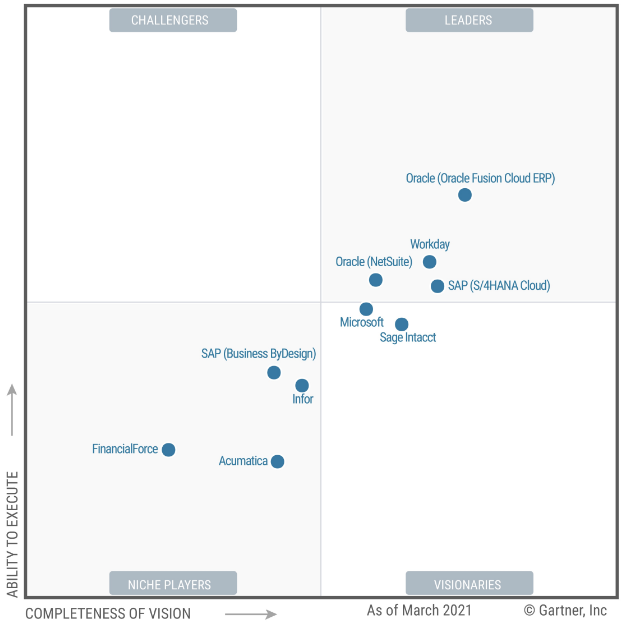
\includegraphics[width=0.5\textwidth]{01/magicQuadrant.png}
                \caption{Magic Quadrant di Gartner. Source: (Maggio 2021) Gartner}
            \end{figure}
\section{Long Tail di Anderson}
    La \textbf{Long Tail} è un modello sviluppato da \textbf{Chris Anderson} che rappresenta la \textbf{distribuzione delle vendite} di un prodotto (non per forza informatico o di nuova tecnologia). Questo modello descrive come la vendita di una certa categoria di prodotti è distribuita tra i prodotti più venduti e i prodotti meno venduti.
    L'effettiva ``\textbf{coda lunga}'' è la parte della distribuzione delle vendite che si trova dopo i prodotti più venduti. Questa parte della distribuzione è composta da molti prodotti che vendono poche copie ciascuno.
    \paragraph{Conseguenze} Questo modello ha diverse conseguenze:
        \begin{itemize}
            \item \textbf{Aumento della varietà} di prodotti disponibili sul mercato.
            \item \textbf{Aumento della disponibilità} di prodotti di nicchia.
            \item \textbf{Aumento della vendita} di prodotti di nicchia.
            \item \textbf{Aumento della vendita} di prodotti meno popolari.
            \item \textbf{Aumento della vendita} di prodotti meno venduti.
        \end{itemize}
        Conseguenza fondamentale riguarda soprattutto i motori online, in quanto questi possono permettersi di vendere prodotti di nicchia in quanto non hanno i costi di un negozio fisico.
        \begin{figure}[H]
            \centering
            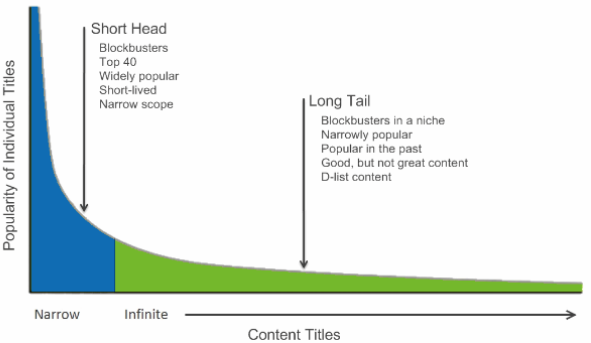
\includegraphics[width=0.5\textwidth]{01/longTail.png}
            \caption{Long Tail}
        \end{figure}
